\documentclass[12pt,letterpaper,boxed]{hmcpset}
\usepackage[margin=1in,headheight=14pt]{geometry}
\usepackage{amsfonts, amsmath, amssymb, enumerate, fancyhdr, gensymb, lastpage, mathtools, parskip, graphicx}
\usepackage{xcolor, tikz-cd}
\newcommand{\wg}[1]{\textcolor{violet}{#1}}
\newcommand{\OO}{\mathcal O}
\newcommand{\Q}{\mathbb Q}
\newcommand{\R}{\mathbb R}
\newcommand{\C}{\mathbb C}
\newcommand{\Z}{\mathbb Z}
\newcommand{\abs}[1]{\left|#1\right|}
\newcommand{\im}{\text{im }}
\newcommand{\inv}{^{-1}}
\newcommand{\normal}{\unlhd} %% one can also use \trianglelelefteq
\newcommand{\anglee}[1]{\langle #1 \rangle}
\usepackage[shortlabels]{enumitem}

% Numbering macros
\pagestyle{fancy}
\lhead{Will Gilroy}
\chead{Algs Homework \#}
\rhead{03 November 2021}
\lfoot{}
\cfoot{}
\rfoot{Page\ \thepage\ of\ \pageref{LastPage}}

\linespread{1.5}

\newcommand\blankpage{
    \thispagestyle{empty}
    \addtocounter{page}{-1}
    \newpage}
\renewcommand\footrulewidth{0.4pt}

\begin{document}

\problemlist{Algorithms HW } 

%------------------------- Problem 1 -----------------------

\begin{problem}[1]
	\hfill
\end{problem}

\begin{solution}
\end{solution}

\newpage

%------------------------- Problem 2 -----------------------

\begin{problem}[2]
	\hfill
\end{problem}

\begin{solution}
\end{solution}

\newpage

%------------------------- Problem 3 -----------------------

\begin{problem}
	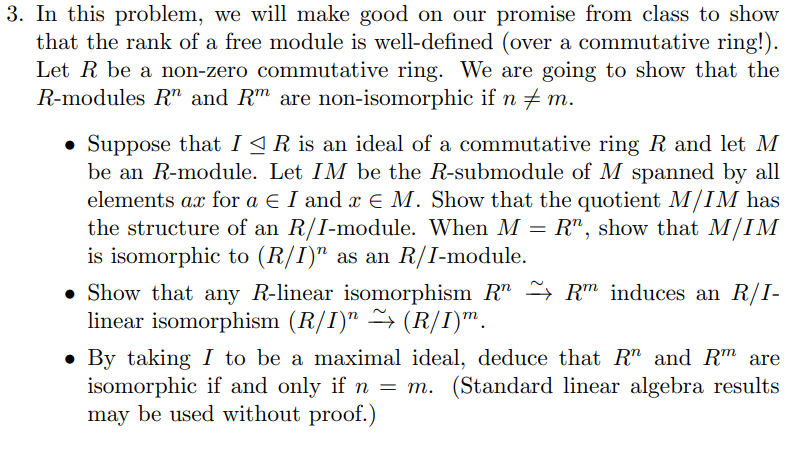
\includegraphics[scale=0.7]{3.png}
	\hfill
\end{problem}
\begin{solution}
\begin{itemize}
\item To show that $M/IM$ has the structure of an $R/I$-module, we
must show that $M/IM$ has an underlying abelian group structure with
respect to addition, and that there is a well-defined $R/I$ scaler
multiplication on $M/IM$.

First, we show that $M/IM$ has a well-defined abelian group structure
with respect to addition. By definition $M$ has an abelian group
structure, and so $IM$ is a normal subgroup of $M$. It follows that
the quotient group $M/IM$ is well-defined and moreover is also
abelian. One way to see that the quotient group is abelian is to
recall that the quotient map $\pi: M \to M/IM$ is a group homomorphism
and so \[
\pi(x) + \pi(y) = \pi(x + y) = \pi(y + x) = \pi(y) + \pi(x),
\]
for all $x,y \in M$. 

Next, we propose an $R/I$ scaler multiplication on $M/IM$. If $r + I
\in R/I$ and $m + IM \in M/IM$. Then I claim that scaler multiplication given
by $(r+I) \cdot (m + IM) := rm + IM$ is well defined.
Let $r + I = r' + I$ be equivalent elements of $R/I$. Then we have
that there's some $a \in I$ such that $r = r' + a$. Now let $m + IM
\in M/IM$ and consider \[
rm + IM = (r' + a)m + IM = r'm + IM + am + IM = r'm + IM + 0 + IM =
r'm + IM,
\]
since $am \in IM$ by definition. That is, our proposed scaler
multiplication maps $m \in M$ to the same class mod $IM$, regardless
of choice of representative of $r + IM$. Hence our multiplication is
well defined and we have found an $R/I$-module structure on $M/IM$.

\item 
Suppose $\phi: R^n \to R^m$ is an $R$-linear isomorphism. Since $R^n$
is a free $R$-module, it follows that $\phi$ is defined exactly by its
action on the basis $\{e_i\}$ where $e_i = (0, \cdots, 1, \cdots 0)$
with the $1$ in the $i$th position.

Now notice that $\bar e_i := \pi(e_i)$ is an $R/I$-basis for
$(R/I)^n$. And so maps out of $(R/I)^n$ can be defined by their action
on $\bar e_i$. We define a map $\bar \phi: (R/I)^n \to (R/I)^m$ by
$\bar \phi(\bar e_i) = (\pi \circ \phi)(e_i)$. This map is $R/I$
linear by construction, we claim that it is also a bijection.

First we show surjectivity. 
Suppose $(\bar b_1, \bar b_2, \cdots, \bar b_m) \in (R/I)^m$. Since
$\pi: R \to R/I$ is a surjection, there is an element $(b_1, b_2,
\cdots, b_m) \in R^m$ such that $\pi(b_1, b_2, \cdots, b_m) = (\bar
b_1, \bar b_2, \cdots, \bar b_m)$. Moreover, $\phi$ is an isomorphism
and so there also exists an element $(a_1, a_2, \cdots, a_n) \in R^n$
such that $\phi(a_1, \cdots, a_n) = (b_1, \cdots, b_m)$. It then
follows that $\bar\phi(\bar a_1, \bar a_2, \cdots, \bar a_n) = (\bar
b_1, \bar b_2, \cdots, \bar b_m)$. Thus, $\bar \phi$ is surjective.

Now consider $0 \in (R/I)^m$. Tuples of the form $(b_1, \cdots, b_m)
\in R^m$ with $b_i \in I$ map to $0$ under $\pi$. Since $\phi$ is an
isomorphism from $R$ to $R$, only elements $(a_1, \cdots, a_n) \in
R^n$ with $a_i \in I$ satisfy $\phi(a_1, \cdots, a_n) = (b_1, \cdots,
b_m)$ with $b_i \in I$. Then, only elements of the form
$(\bar a_1, \bar a_2, \cdots, \bar a_n) \in (R/I)^n$ map to $0 \in
(R/I)^m$ under $\bar \phi$. However, since $a_i \in I$ we have 
$(\bar a_1, \cdots, \bar a_n) = 0 \in (R/I)^n$. And so $\bar \phi$ is
injective.

We have found a bijective $R/I$-linear map $\bar\phi: (R/I)^n \to
(R/I)^m$ and so we have found an induced $R/I$-linear isomorphism
$(R/I)^n \to (R/I)^m$. 

\item 
Suppose $n = m$, then $R^n = R^m$ and so $R^n \cong R^m$ as
$R$-modules.

Now suppose that $R^n \cong R^m$. Since $R$ is a non-zero commutative
ring we have (via the axiom of choice (or perhaps Zorn's lemma)) 
that there exists a maximal ideal $I \normal R$. 
Now by part $(b)$ we have an induced isomorphism on the $R/I$ modules
$(R/I)^n \cong (R/I)^m$. However, since $I$ is maximal, it follows
that $R/I$ is a field and so $(R/I)^n$ and $(R/I)^m$ are in fact
$R/I$-vector spaces. Vector spaces are characterized by their
dimension and so it follows that $(R/I)^n \cong (R/I)^m$ as $R/I$
vector spaces implies $n = m$. 

Hence the rank of a free module over a non-zero commutative ring is a
well defined notion. 

\end{itemize}
\end{solution}

\newpage

%------------------------- Problem 4 -----------------------

\begin{problem}
	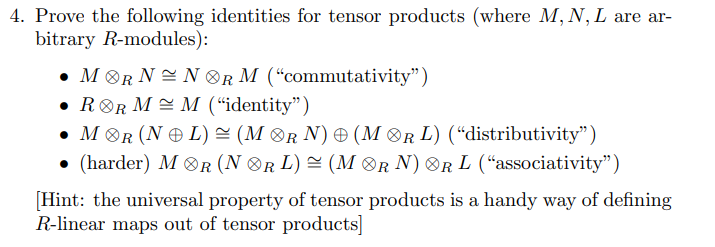
\includegraphics[scale=0.8]{4.png}
	\hfill
\end{problem}

\begin{solution}
\begin{itemize}
\item Consider the map $M \times N \to N \otimes_R M$ given by $((m,n)
\mapsto n \otimes m)$. Notice that this map is $R$-bilinear on $M \times
N$ since $\otimes: M \times N \to M \otimes_R N$ is.
Then by the universal property of tensor products we have a unique
$R$-linear map $f: M \otimes_R N \to N \otimes_R M$ such that $f \circ
\otimes = (m,n) \mapsto n \otimes m$. 
The same argument on the $R$-bilinear map $N \times M \to N \otimes_R
M$ given by $(n,m) \mapsto (m \otimes n)$ gives a unique $R$-linear
map $\tilde f: N \otimes_R M \to M \otimes_R N$ such that\footnote{
The ``$\otimes$'' in the following phrase now refers to the
$R$-bilinear map $N \times M \to N \otimes_R M$, whereas earlier it
referred to the $R$-bilinear map $M \times N \to M \otimes_R N$.
} $\tilde f
\circ \times = (n,m) \mapsto m \otimes n$. 

Notice now that $f \circ \tilde f = id_{N \otimes_R M}$ and $\tilde f
\circ f = id_{M \otimes_R N}$. Indeed $(f \circ \tilde f)(m \otimes n)
= f(n \otimes m) = m \otimes n$. And likewise for the other direction.

That is, we have found a bijective $R$-linear map $M \otimes_R N \to N
\otimes_R M$ and so in fact $M \otimes_R N$ is isomorphic to $N
\otimes_R M$.


\item Consider the following map $M \times N \to M$ via $(r,m) \mapsto
rm$ given by the module structure on $M$. Notice that this map is
bilinear \wg{come back and write the computation out}
And so by the universal property of tensor products we have a unique
$R$-linear map $f: R \otimes_R M \to M$ such that $r \otimes n
\mapsto rm$. 

I claim that this map is bijective and so is an isomorphism of
$R$-modules. First notice that $f$ is surjective. Indeed, if $m \in M$
then $f(1 \otimes m) = 1\cdot m = m$, so long as $R$ is not the zero
ring. If $R$ is the zero ring, then $M$ must be the zero module, and
then our desired isomorphism trivially holds. 

Next we show that $f$ is injective. 
Suppose we have $r \cdot m' = m$ for some $m,m' \in M$ and
$r \in R$. Then notice 
\[
	r \otimes m' = 1 \cdot r \otimes m' = r
		\otimes r \cdot m' = 1 \otimes m,
\]
And so $rm' = m$ implies $r \otimes m' = 1 \otimes m$. This suffices
to show that $f$ is injective because if generally we have $r_1 m_1 =
r_2 m_2$ then by definition $r_1 m_1 = m'$ for some $m' \in M$ and
then we have $m' = r_2 m_2$. 

Overall we have a bijective $R$-linear map $R \otimes_R M \to M$, and
so $R \otimes_R M \cong M$.

\item 
First we acquire an $R$-linear map $M \otimes_R (N \oplus L) \to (M
\otimes_R N) \oplus (M \otimes_R L)$ by leveraging the universal
property of tensor products. And then we show that this map is in fact
an isomorphism.

First define a map $h: M \times (N \oplus L) \to (M \otimes_R N)
\oplus (M \otimes_R L)$ by $h(m, (n,l)) = (m \otimes n, m \otimes l)$. 
Note that in $R$-Mod finite coproducts are also products, and so the
domain of the function $h$ is the $R$-module $M \oplus N \oplus L$.
We claim that this map is $R$-bilinear. 
Consider
\begin{align*}
	h(r_1 m_1 + r_2 m_2, (n,l)) 
		&= ((r_1m_1 + r_2m_2) \otimes n , (r_1m_1 + r_2 m_2) \otimes l) \\
		&= (r_1(m_1 \otimes n) + r_2 (m_1 \otimes n), r_1(m \otimes l) + r_2(m_2 \otimes n)) \\
		&= r_1(m_1 \otimes n, m_1 \otimes l_1) + r_2(m_2 \otimes n, m_2 \otimes l).
\end{align*}
By the definition of the tensor product relations, and of the
$R$-module structure on the direct sum of two $R$-modules. In other
words, we have shown that $h$ is $R$-linear in the first argument. Now
consider the second argument
\begin{align*}
	h(m, r_1(n_1, l_1) + r_2(n_2, l_2)) 
		&= (m \otimes r_1 n_1 + r_2 n_2, m \otimes r_1 l_1 + r_2 l_2) \\ 
		&= (r_1 (m\otimes n_1) + r_2 (m \otimes n_2), r_1(m \otimes l_1) + r_2(m \otimes l_2)) \\
		&= r_1(m \otimes n_1, m \otimes l_1) + r_2(m \otimes n_2, m \otimes l_2), 
\end{align*}
using the bilineararity of the tensor product, and by using the
definition of the $R$-module structure on the direct sum of
$R$-modules. That is, we've shown $h$ is $R$-linear in the second
argument also. And so $h$ is an $R$-bilinear map.

We are now free to use the universal property of tensor products to
acquire a new $R$-linear map $f: M \otimes_R (N \oplus L) \to (M
\otimes_R N) \oplus (M \otimes_R L)$. where $f(m \otimes (n,l)) = (m \otimes
n, m \otimes l)$. If we can verify that this map is bijective then we
are done. 

First we show $f$ is surjective. Let $(m \otimes n, m \otimes l) \in
(M \otimes_R N) \oplus (M \otimes_R L)$ then we have $m \otimes (n,l)
\in M \otimes_R (N \oplus L)$ maps to the desired element.

Now suppose $f(m \otimes (n,l)) = 0$ that is $m \otimes n = 0$ and $m
\otimes l = 0$. We want to show that $m \otimes (n,l) = 0$.
\wg{come back to this. There might be another way to do this using the
universal property of tensor products}





\end{itemize}
\end{solution}

\newpage

%------------------------- Problem 5 -----------------------

\begin{problem}[4]
	\hfill
\end{problem}

\begin{solution}
\end{solution}

\newpage

%------------------------- Problem 6 -----------------------

\begin{problem}
	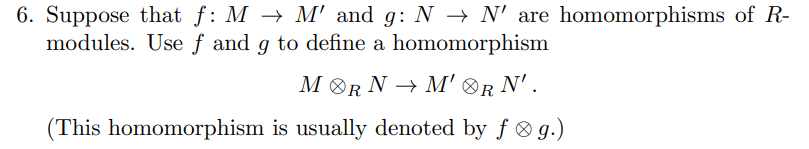
\includegraphics[scale=0.7]{6.png}
	\hfill
\end{problem}

\begin{solution}
We define the desired map by using the universal property of tensor
products.
Consider the following composition
\[
	M \oplus N \xrightarrow{(f,g)} M' \oplus N'  \xrightarrow{\otimes} M' \otimes_R N',
\]
via 
\[
	(m,n) \mapsto (f(m), g(n)) \mapsto f(m) \otimes g(n).
\]
We claim that this composition $\phi: M \oplus N \to M \otimes_R N$ is
$R$-bilinear. Indeed, first let $n \in N$ be fixed and then consider
\begin{align*}
	\phi(r_1 m_1 + r_2 m_2, n)  
		&= (r_1 f(m_1) + r_2 f(m_2)) \otimes g(n) \\
		&= (r_1 f(m_1)) \otimes g(n) + (r_2 f(m_2)) \otimes g(n) \\
		&= r_1(f(m_1) \otimes g(n)) + r_2 (f(m_2) \otimes g(n)) \\
		&= r_1 \phi(m_1, n) + r_2 \phi(m_2, n), 
\end{align*}
by the relations on the elements of the tensor product. In other
words, we have shown that $\phi(-, n)$ is $R$-linear for each $n \in N$. A very similar
calculation will show that $\phi(m, -)$ is $R$-linear for each $m \in
M$. That is, $\phi$ is $R$-bilinear.

By the universal property of the tensor product we then have an
$R$-linear map $\psi: M \otimes_R N \to M' \otimes_R N$ given by $m
\otimes n \mapsto f(m) \otimes g(n)$, as desired. 

\end{solution}

\newpage

%------------------------- Problem 7 -----------------------

\begin{problem}
	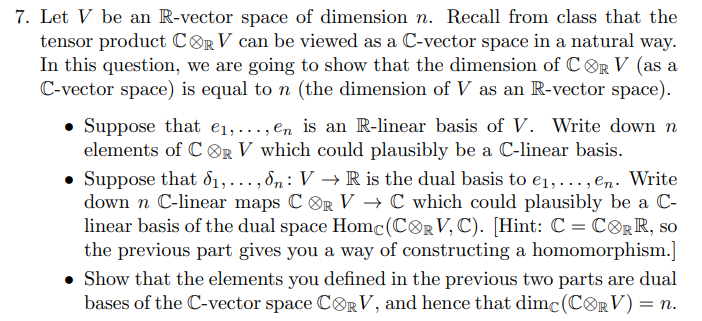
\includegraphics[scale=0.8]{7.png}
	\hfill
\end{problem}

\begin{solution}
\item I claim that $1 \otimes e_1, 1 \otimes, e_2, \cdots, 1 \otimes
e_n \in \C \otimes_\R V$ is a basis. First we show that these tensors
span $\C \otimes_\R V$. First let $\alpha \otimes v \in \C \otimes_\R
V$ be a pure tensor. Then, since $\{e_i\}$ is a basis for $V$ we have
$v = \lambda_1 e_1 + \cdots \lambda_n e_n$ for $\lambda_i \in \R$.
Now notice 
\begin{align*}
	\alpha\lambda_1(1 \otimes e_1) + \alpha\lambda_2(1 \otimes e_2)
		+ \cdots + \alpha\lambda_n(1 \otimes e_n) 
	&= \alpha 
	\left[ 1 \otimes \lambda_1 e_1 + 1 \otimes \lambda_2 e_2 + \cdots 1 \otimes \lambda_n e_n \right] \\
	&=  \alpha \otimes (\lambda_1 e_1 + \cdots + \lambda_n e_n) \\
	&=  \alpha \otimes v.
\end{align*}
That is, every pure tensor in $\C \otimes_R V$ is a finite $\C$-linear
combination of the $1 \otimes e_i$. It then follows that every element
of $\C \otimes_\R V$, which is a finite $\C$-linear combination of
pure tensors, is also a finite $\C$-linear combination of the $1
\otimes e_i$. Thus, the $1 \otimes e_i$ span $\C \otimes_R V$ over
$\C$. 

I will show some approximation of the $1 \otimes e_i$ being
$\C$-linearly independent. Suppose we have $a_1(1 \otimes e_1) +
\cdots + a_n(1 \otimes e_n) = 0$ for some $a_i \in \R$. Then, we have
\begin{align*}
	0 &= a_1(1 \otimes e_1) + a_2(1 \otimes e_2) + \cdots + a_n(1 \otimes e_n) \\
	&= 1 \otimes (a_1 e_1 + a_2 e_2 + \cdots + a_n e_n) = 0 \\
	&\implies a_1 e_1 + a_2 e_2 + \cdots + a_n e_n = 0 \\
	&\implies a_i = 0 \text{ for all $i$,}
\end{align*}
where the last line follows since the $e_i$ are an $\R$-linear basis
for $V$, and so are $\R$-linearly independent. The second to last line
follows since $1 \neq 0 \in \C$. 
This shows that the elements $1 \otimes e_i$ are $\R$-linearly
independent. This argument does not work for $a_i \in \C$, becuase we
are unable to ``bring the coefficients into the second `coordinate'
of the pure tensors.'' That is, we do not have a $\C$-vector space
structure on $V$ exactly.

\item We want to study the $\C$-linear maps 
$\C \otimes_\R V \to \C = \C \otimes_\R \R$. We first consider maps
which descend from bilinear maps $C \times V \to  \C \otimes_\R \R$
induced by $f \in V^*$.
First, fix a map $f \in
V^\star$. And then we define a map $\phi_f: \C \times V \to  \C
\otimes_\R \R$ via $\phi_f(\alpha, v) = \alpha \otimes f(v)$.
First notice that this map is $\R$-linear in the second coordinate: if
we fix $\alpha \in \C$ and let $a_1, a_2 \in \R$ indeed, we have \[
\phi_f(\alpha, a_1v_1 + a_2 v_2) = \alpha \otimes f(a_1 v_1 + a_2 v_2)
	= \alpha \otimes (a_1 f(v_1) + a_2 f(v_2)) 
	= a_1(\alpha \otimes f(v_1)) + a_2(\alpha \otimes f(v_2)), 
\]
Since $f$ is an $\R$-linear map and by the bilinearity of the tensor
product.
A similar calculation shows that $\phi_f$ is $\C$-linear in the first
coordiante.

Now, since $\delta_1, \cdots, \delta_n$ is a basis for $V^*$ then we
can represent $f(v) = a_1 \delta_1(v) + a_2 \delta_2(v) + \cdots a_n
\delta_n(v)$ for $a_i \in \R$. Then we can represent
\[
\phi_f(\alpha, v) = \alpha \otimes (a_1\delta_1(v) + \cdots + a_n \delta_n(v))
	= \alpha a_1 (1 \otimes \delta_1(v)) + \alpha a_2 (1 \otimes \delta_2(v)) +
		\cdots + \alpha a_n (1 \otimes \delta_n(v)),
\]
Note that the $a_i$ in the computation above depends only on the map
$f \in V^*$. 
This suggests that a plausible basis for $Hom_\C(\C \otimes_\R V, \C)$
could be the maps $1 \otimes \delta_i \in Hom_\C(\C \otimes_\R, \C).$

\wg{is there more that we can show?}




\end{solution}

\newpage

%------------------------- Problem 8 -----------------------

\begin{problem}[4]
	\hfill
\end{problem}

\begin{solution}
\end{solution}

\newpage



\end{document}
